% Partie VI condensée (FR). Figures recopiées, labels et captions traduits ; le cas
% publié source reste en anglais (source PubMed réelle). Tables à colonnes S : les
% virgules décimales sont posées automatiquement par siunitx (préambule FR).

\noindent Une étude clinique tient un formulaire structuré pour chacun de ses patients, le
formulaire de recueil électronique, ou eCRF. Il contient une ligne par patient, avec
un ensemble fixe de champs comme le traitement administré ou sa date de début, et il
est rempli à partir des comptes-rendus du patient.

Pour en faire des systèmes utiles, nous abordons la tâche qui motive cette thèse :
extraire de documents cliniques des variables propres à chaque étude. Chaque projet
demande des champs différents, généralement avec peu ou pas de données annotées. Aucun
jeu de données ouvert n'associe un dossier hospitalier français à un formulaire rempli
par un clinicien, et les dossiers eux-mêmes ne peuvent quitter l'hôpital, la
supervision doit donc être construite plutôt que collectée. Nous utilisons de grands
modèles de langue pour annoter du texte public, pour juger des types jamais observés
quand les références fixes font défaut, et pour générer des dossiers synthétiques de
lymphome dérivés de cas cliniques publiés dans des articles scientifiques. Les deux
voies utilisent Qwen3-235B avec une sortie JSON contrainte, et les annotations
obtenues sont automatiques, dites \textit{silver}, plutôt que produites par des humains.

\begin{center}
\begin{minipage}{\linewidth}
  \centering
  \resizebox{\textwidth}{!}{%
  \begin{tikzpicture}[
    font=\small, text=ThesisInk, >={Stealth[length=2mm]},
    box/.style={draw=ThesisNeutral, fill=ThesisPaper, rounded corners=3pt,
                text width=4.6cm, minimum height=3.8cm, inner sep=9pt, align=left},
    doc/.style={box, font=\small\itshape, text width=6.4cm},
    lbl/.style={font=\scriptsize, text=ThesisInk},
    arr/.style={->, draw=ThesisNeutral, line width=0.7pt, shorten >=5pt, shorten <=5pt}]
    \node[doc] (case) at (-6.8,0) {%
      A 56 year old male patient was diagnosed with a diffuse large B-cell
      lymphoma (DLBCL). He was treated by six cycles of rituximab,
      cyclophosphamide, hydroxydaunorubicin, vincristine, and prednisolone
      (R-CHOP), followed by two cycles of rituximab. He developed a relapse of a
      composite lymphoma. Therapy with rituximab, dexamethasone, cytarabine, and
      cisplatin (R-DHAP) was initiated.};
    \node[box] (timeline) at (0,0) {\textbf{Chronologie structurée}\\[6pt]
      \textcolor{ThesisPrimaryDark}{2018} · diagnostic, DLBCL\\
      \textcolor{ThesisPrimaryDark}{2018} · R-CHOP, six cycles\\
      \textcolor{ThesisPrimaryDark}{2019} · rituximab, deux cycles\\
      \textcolor{ThesisPrimaryDark}{2020} · rechute\\
      \textcolor{ThesisPrimaryDark}{2020} · R-DHAP};
    \node[box] (reports) at (5.8,0) {\textbf{Comptes-rendus français générés}\\[6pt]
      \textcolor{ThesisPrimaryDark}{18 mai 2018} · anatomopathologie\\
      \textcolor{ThesisPrimaryDark}{22 mai 2018} · RCP\\
      \textcolor{ThesisPrimaryDark}{14 janvier 2019} · imagerie\\
      \textcolor{ThesisPrimaryDark}{25 avril 2020} · consultation de rechute};
    \node[lbl, above=2pt of case.north] {Cas publié, PubMed Central};
    \draw[arr] (case) -- (timeline);
    \draw[arr] (timeline) -- (reports);
  \end{tikzpicture}}
  \captionof{figure}{Un vrai cas publié, à gauche, et les deux étapes qui le
  transforment en un dossier longitudinal daté.}
  \label{fig:p3-case-to-record}
\end{minipage}
\end{center}
\medskip

La \Cref{fig:p3-case-to-record} montre l'un de ces cas et ce que nous en faisons : un
cas publié devient un dossier longitudinal daté, un substitut synthétique de la
séquence de comptes-rendus à partir de laquelle un formulaire d'étude est rempli.

La génération suit la chronologie clinique. Nous convertissons d'abord le cas source
en une frise temporelle française structurée, puis nous générons les documents cliniques un
à un, en réextrayant la frise après chaque génération comme contrôle de cohérence,
de sorte qu'un compte-rendu à une date donnée ne reçoive que les événements déjà
survenus. Le corpus obtenu contient 2\,050 dossiers longitudinaux, chacun avec une
médiane de huit documents et de 22\,314 caractères, et 31\% d'entre eux
comportent une deuxième ligne de traitement. En faire un jeu d'entraînement pour l'extraction est
l'étape suivante : chaque valeur doit être reliée à l'un des 89 champs du
formulaire qui nous intéresse et localisée dans le dossier complet. Une dernière passe du modèle de
langue sur 16\,375 comptes-rendus produit 237\,194 annotations reliant des segments de
texte à ces champs. La référence est automatique plutôt qu'humaine. La même famille
de modèles génère les dossiers et propose leurs
étiquettes, ce qui peut favoriser les conventions du générateur plutôt que la vérité
clinique.

La chaîne de génération a été affinée avec le retour de cliniciens en exercice de CHU
français. À travers une interface d'annotation web et des échanges en visioconférence,
ils ont examiné des versions successives des dossiers synthétiques, en jugeant à la
fois la qualité des annotations automatiques et le réalisme du texte généré, et leurs
remarques ont nourri les versions suivantes. Cette relecture a façonné les dossiers
mais est restée informelle. Une évaluation structurée et reproductible du réalisme
clinique, avec un protocole défini et un panel de cliniciens, reste à mener.

La supervision générée entraîne des extracteurs compacts à vocabulaire ouvert, dont
les descriptions des champs cibles sont fournies en texte à l'inférence. Sur un jeu
d'évaluation eCRF synthétique, notre plus petit modèle adapté à la tâche dépasse les
questions-réponses extractives et se situe à 0,018 de value-$F_1$ du meilleur
générateur affiné, un modèle vingt-sept fois plus grand ; une variante adaptée à la
tâche comble entièrement l'écart, 0,657 contre 0,658. L'adaptation est aussi efficace
en données : la value-$F_1$ passe de 0,182 avec dix dossiers générés à 0,485 avec
cinquante et 0,659 avec l'ensemble d'entraînement complet.

\begin{figure}[ht]
  \centering
  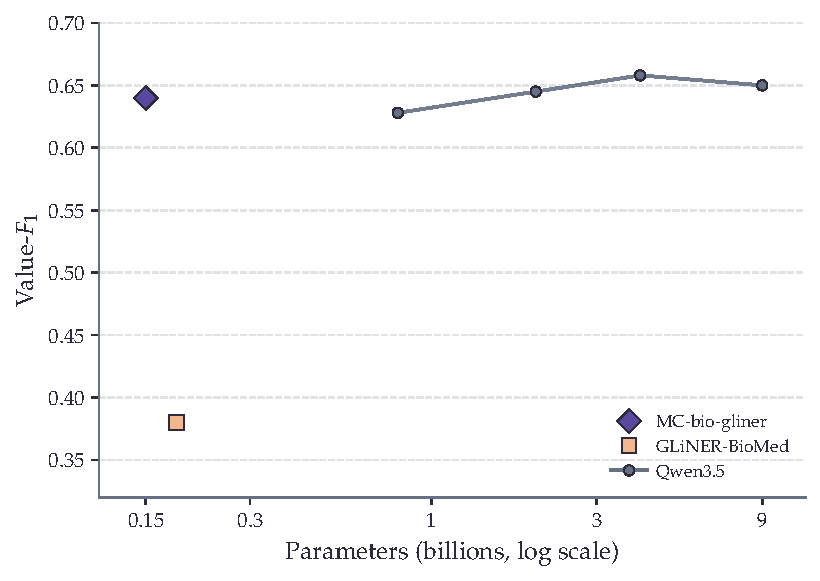
\includegraphics[width=0.82\textwidth]{plots/part_3/output/money_params_vs_f1.pdf}
  \caption{Value-$F_1$ sur l'eCRF du lymphome en fonction du nombre de paramètres,
  après compétition des champs. MC-bio-gliner, à 150 millions de paramètres, se situe
  à 0,018 de value-$F_1$ du meilleur générateur Qwen3.5-4B avec 27 fois moins de
  paramètres, tandis que la référence GLiNER-BioMed de taille comparable, affinée sur
  les mêmes dossiers, reste loin derrière.}
  \label{fig:p3-money}
\end{figure}

La \Cref{fig:p3-money} place chaque système sur l'axe des paramètres. L'encodeur
adapté à la tâche atteint le niveau d'un générateur de quatre milliards de paramètres,
et faire passer ce générateur à neuf milliards n'aide pas. Les générateurs gardent l'avantage
sur le span-$F_1$, jusqu'à 0,567 contre 0,503 pour MC-bio-gliner, et parmi ses erreurs
l'encodeur affecte une valeur correcte au mauvais champ 48,9\% du temps, contre 38,8\%
pour le meilleur générateur : davantage de ses fautes sont des confusions de rôle, la
bonne chaîne placée dans le mauvais champ.

L'écart de taille est aussi un écart de déploiement. La confidentialité et le RGPD
tiennent les dossiers d'un hôpital à l'écart de toute API externe, et la seule
alternative sur site, un générateur de plusieurs milliards de paramètres, ne tient pas
sur le matériel modeste d'un service clinique. L'encodeur, lui, y tient : il tourne là
où les données restent.

L'eCRF synthétique mesure la tâche complète mais ne peut établir le transfert vers du
texte écrit par des humains. Sur des jeux de NER humains (PARHAF, FRACCO), l'avantage
se restreint d'ailleurs à la tâche de remplissage longitudinal pour laquelle
l'extracteur a été construit : sur une NER dense et plate, une référence de taille
comparable reprend le dessus. Tous les éléments de cette évaluation sont synthétiques
ou annotés automatiquement, sans aucun dossier hospitalier réel ni annotation humaine
dans la tâche. Il reste donc à établir si le résultat se transfère aux dossiers écrits
par des humains,
étape nécessaire avant tout usage clinique.
